\section{Leitungsbeläge}

\subsection{Elektrisches und magnetisches Feld}
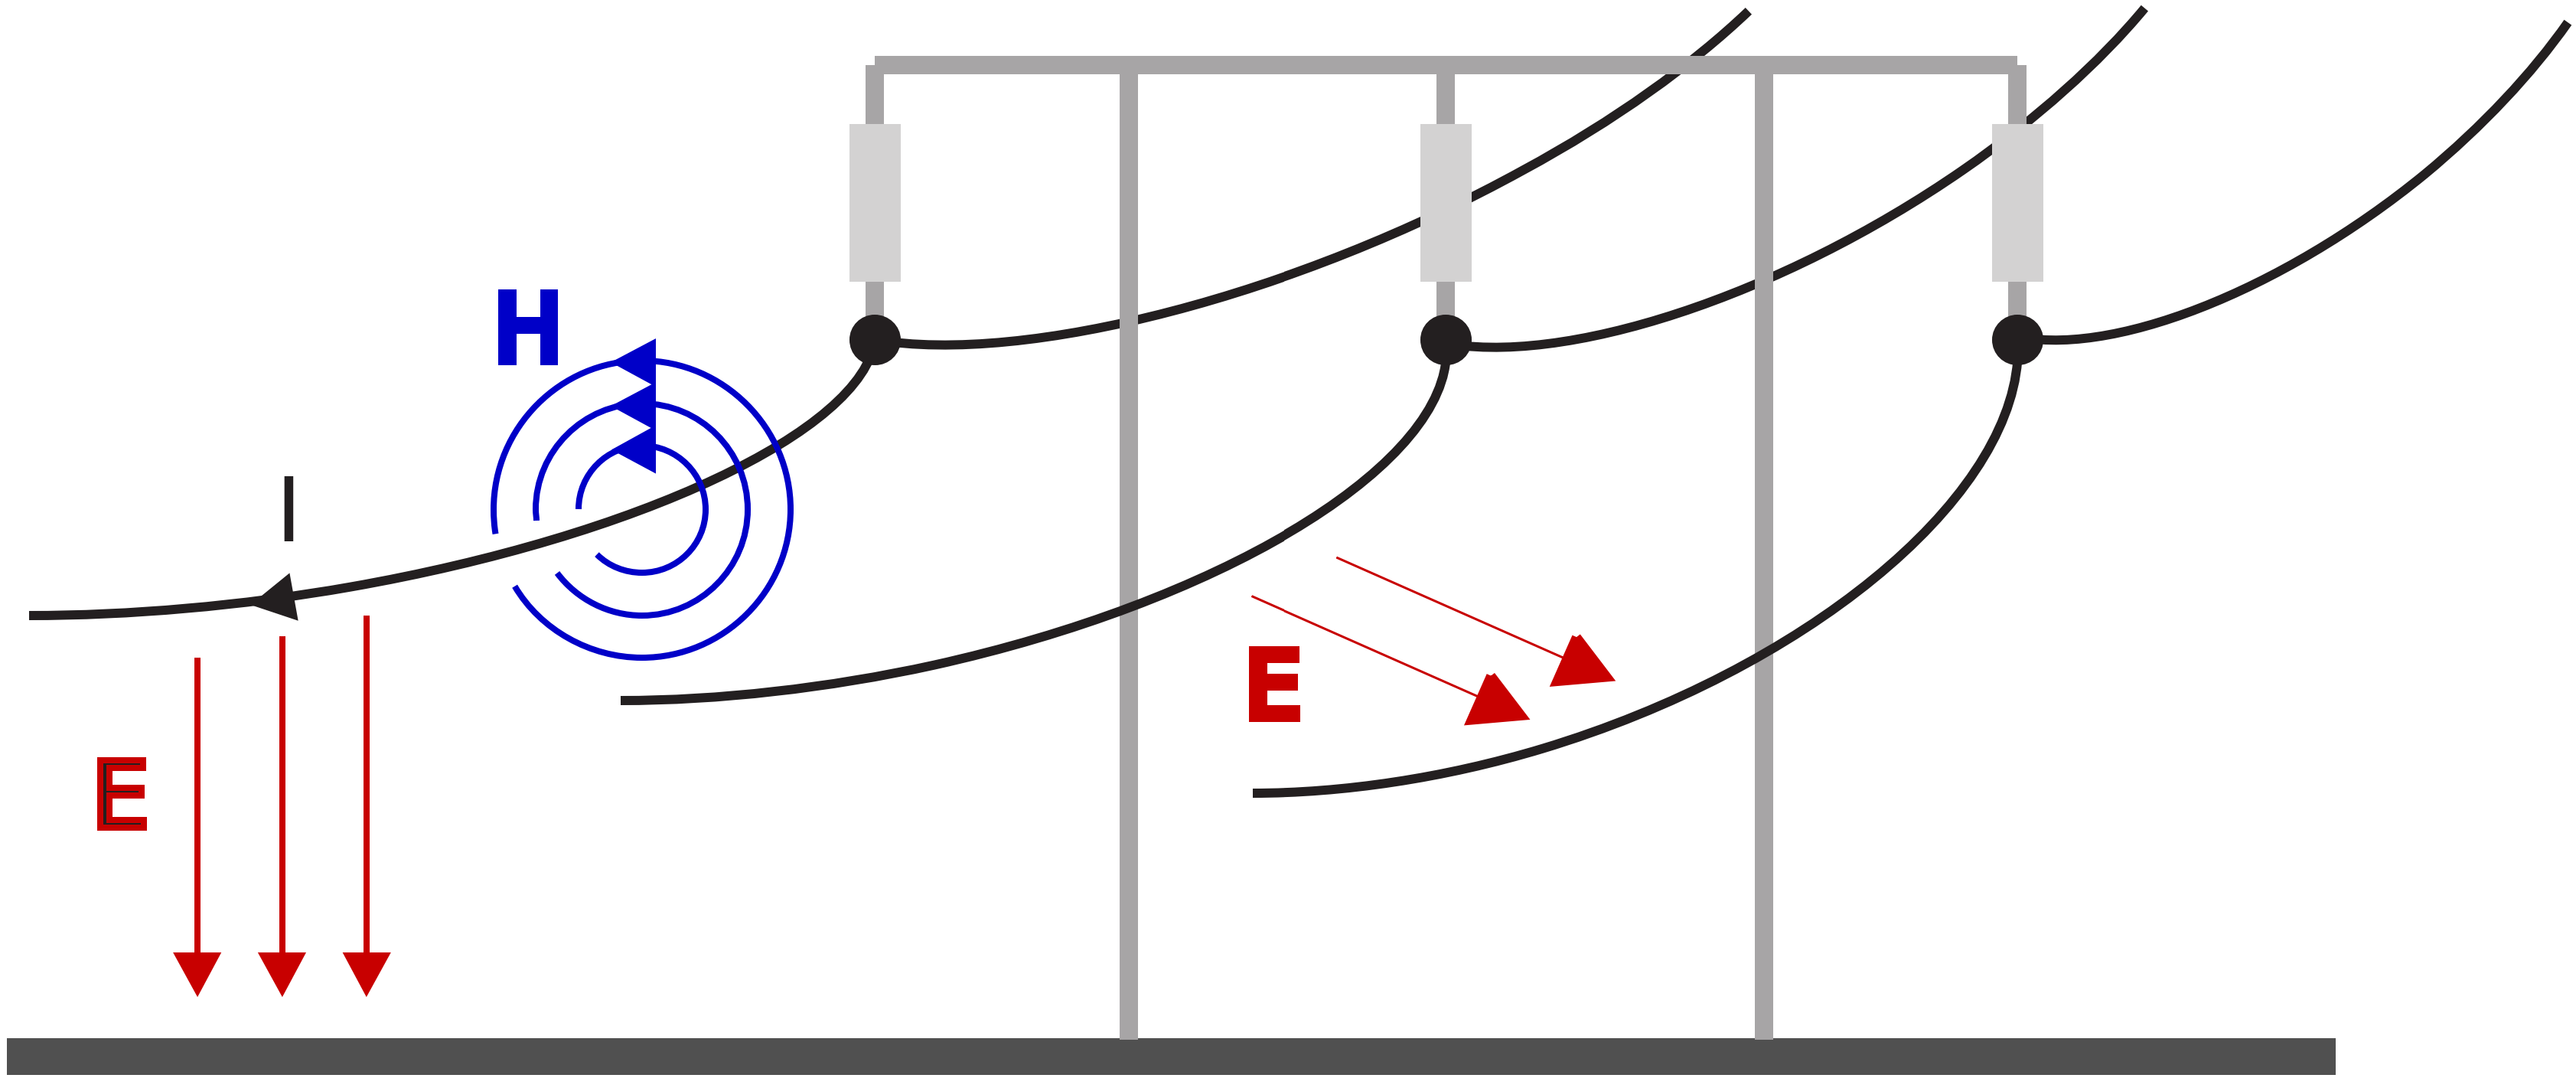
\includegraphics[width=0.98\columnwidth, align=c]{images/Elektrisches_und_Magnetisches_Feld.png}

\subsubsection{Ersatzschaltbild}

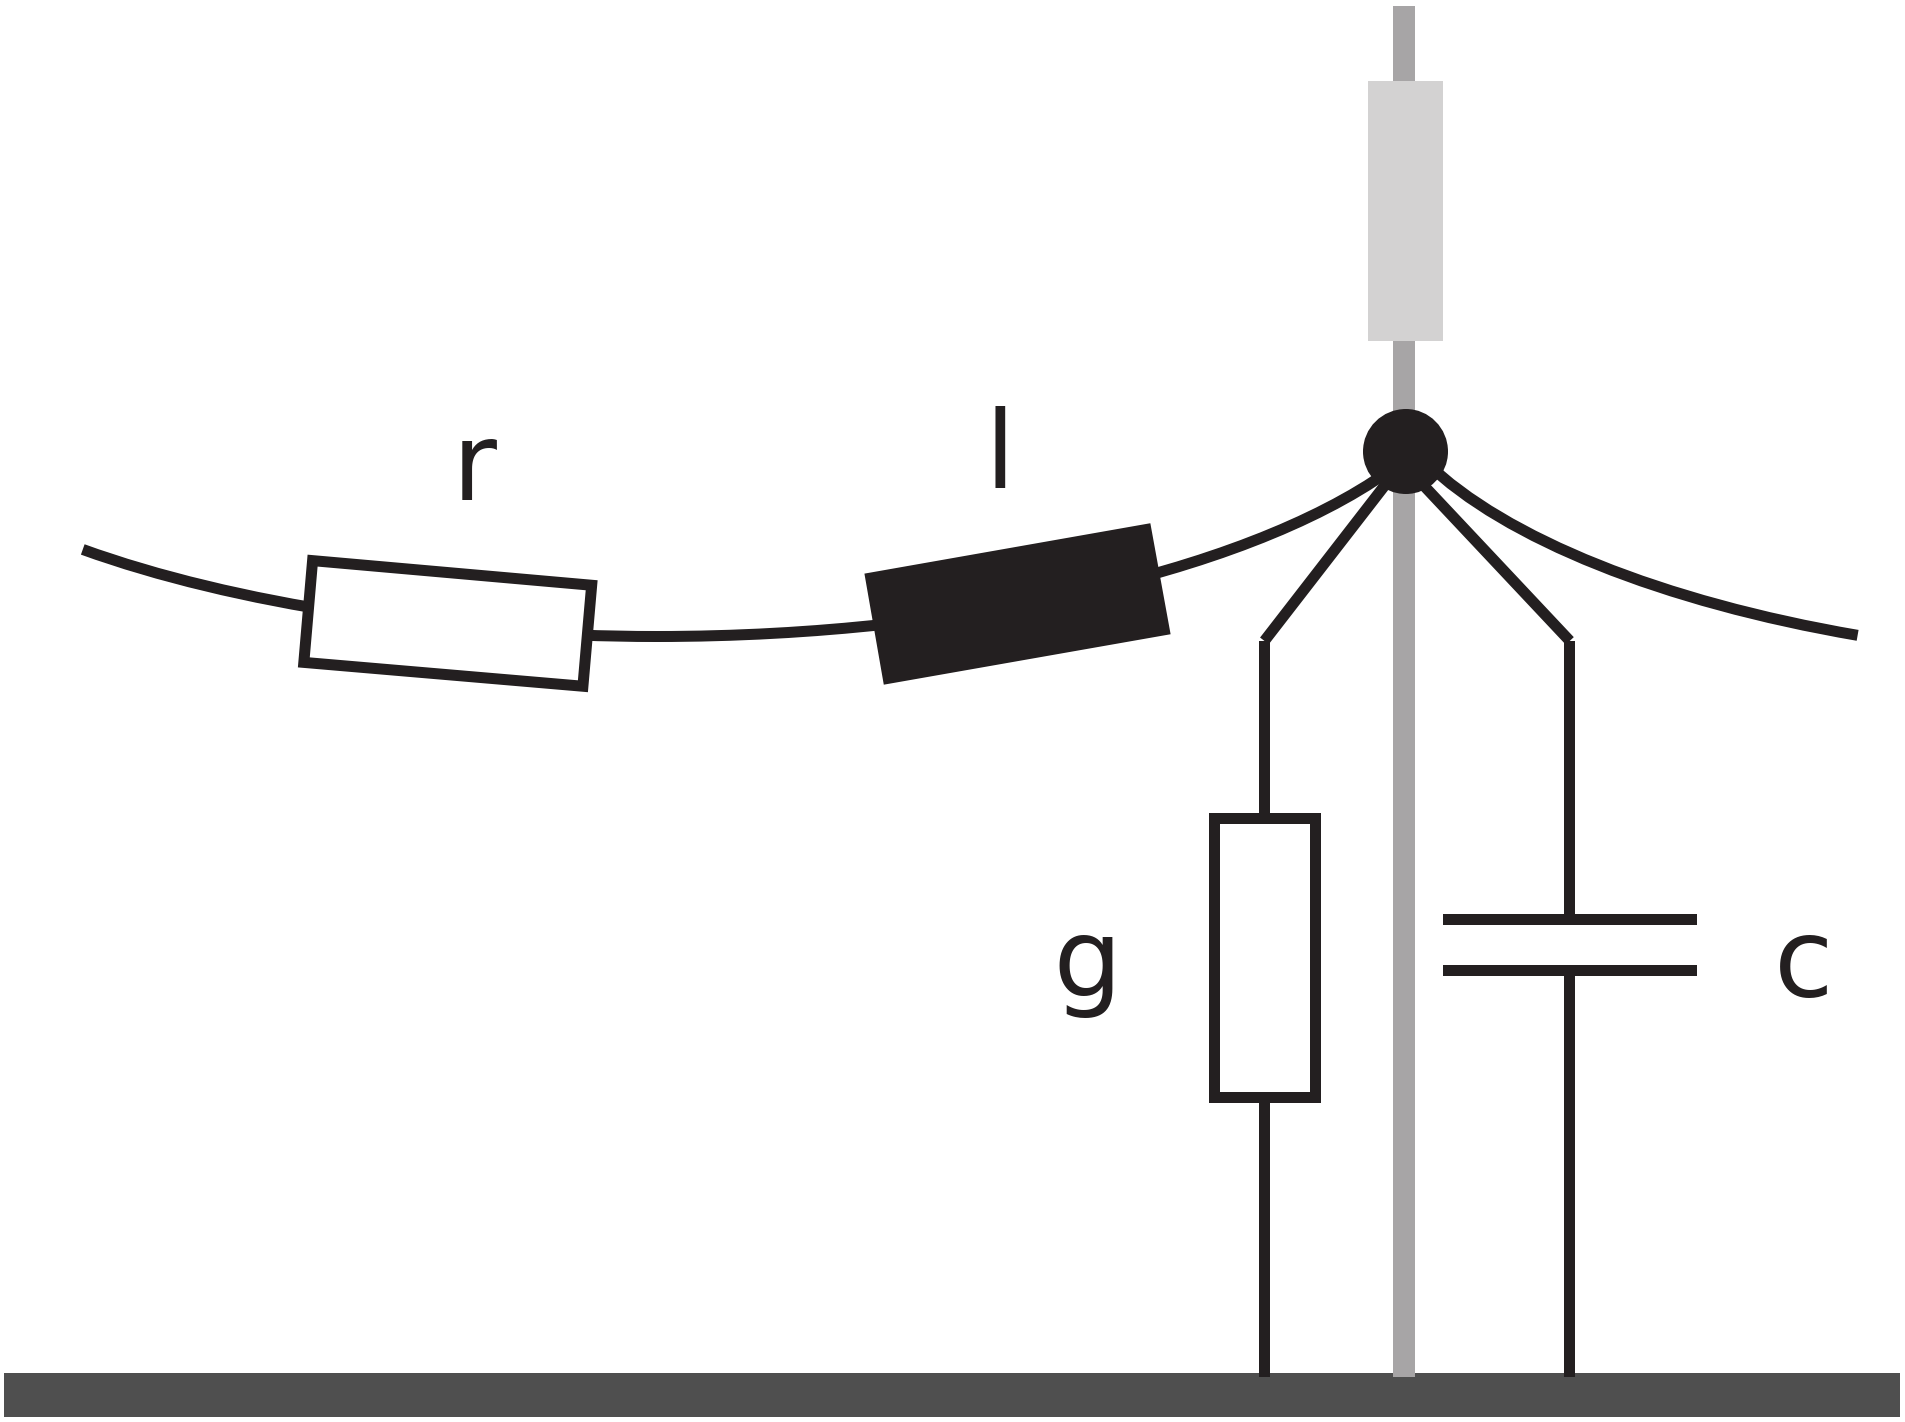
\includegraphics[width=0.55\columnwidth, align=c]{images/Ersatzschaltbild.png}


\subsection{Widerstandsbelag}

\subsubsection{Ursache}
\begin{itemize}
    \item Ohmscher Widerstand des Leiterseils
    \item Bei \textbf{Wechselstrom} $\Rightarrow$ Berücksichtigung der \textbf{Stromverdrängung} (\textit{skin-effect})
\end{itemize}


\subsubsection{Temperaturabhängigkeit des Widerstands}

Der spezifische Widerstand $\rho$ ist temperaturabhängig und ergibt sich aus:

\vspace{0.15cm}

$
\boxed{
\rho = \rho_{20^\circ} \cdot \left[ 1 + \alpha \cdot (T - 20^\circ) \right]
}
$

\vspace{0.15cm}

\renewcommand{\arraystretch}{1.2}
\begin{tabular}{@{} l p{6cm} l @{}}
    $[\rho]$              & Spezifischer Widerstand \dotfill & $\frac{\Omega \cdot \text{mm}^2}{\text{m}}$ \\
    $[\rho_{20^\circ}]$   & Spezifischer Widerstand bei $20\,^\circ$C \dotfill & $\frac{\Omega \cdot \text{mm}^2}{\text{m}}$ \\
    $[\alpha]$            & Temperaturkoeffizient \dotfill & $\frac{1}{\text{$^\circ$C}}$ \\
    $[T]$            & Temperatur \dotfill & $^\circ$C \\
\end{tabular}


\subsubsection{Ohmscher Widerstand des Leiterseils}

Der spezifische Widerstand $R'$ eines Leiterseils in $\frac{\Omega}{\text{m}}$ ergibt sich zu:

\vspace{0.15cm}

$
\boxed{
R' = \sigma \cdot \frac{\rho}{A}
}
$

\vspace{0.15cm}

\renewcommand{\arraystretch}{1.2}
\begin{tabular}{@{} l p{6cm} l @{}}
    $[R']$      & Ohmscher Widerstand pro Meter \dotfill & $\Omega/\text{\text{m}}$ \\
    $[\sigma]$  & Verseilfaktor (typisch $\sigma = 1{,}07$) \dotfill & $-$ \\
    $[\rho]$    & Leitfähigkeit (spezifischer Widerstand) \dotfill & $\frac{\Omega \cdot \text{mm}^2}{\text{m}}$ \\
    $[A]$       & Leiterquerschnitt \dotfill & $\text{mm}^2$ \\
\end{tabular}



\subsection{Skin-Effekt}

Die Eindringtiefe $\delta$ des elektrischen Feldes in einen Leiter ergibt sich zu:

\vspace{0.15cm}

$
\boxed{
\delta = \sqrt{\frac{2 \cdot \rho}{\omega \cdot \mu}}
}
\quad
\boxed{
\delta = \sqrt{\frac{2 \cdot \rho}{2 \cdot \pi \cdot f \cdot \mu}}
}
$

\vspace{0.15cm}

\renewcommand{\arraystretch}{1.2}
\begin{tabular}{@{} l p{6cm} l @{}}
    $[\delta]$   & Eindringtiefe des Stroms (Skin-Tiefe) \dotfill & $\text{m}$ \\
    $[\rho]$     & Spezifischer Widerstand des Leitermaterials \dotfill & $\Omega \cdot \text{m}$ \\
    $[\omega]$   & Kreisfrequenz \dotfill & $\frac{\text{rad}}{\text{s}}$ \\
    $[\mu]$      & Permeabilität des Leitermaterials \dotfill & $\frac{\text{H}}{\text{m}}$ \\
\end{tabular}

\vspace{0.5em}

\textbf{Hinweis:}\\
Bei \textbf{Bündelleitern} wird der Skin-Effekt durch die Aufspaltung des Querschnitts \textbf{abgeschwächt}.



\subsection{Ableitungsbelag}

\begin{itemize}
    \item \textbf{Ursache:} die Verluste des Dielektrikums zwischen den Leitern und zwischen Leiter und Erde
    \item $G'$ ist sehr klein und kann bei normalen Betriebsverhältnissen gegenüber $\omega C'$ \textbf{vernachlässigt} werden
    \item $G'$ ist grösser wenn Teilentladungen (Corona-Effekt) auftreten.
    \item \textbf{Witterungsabhängig}
  \end{itemize}


\newcolumn
\subsection{{Induktivitätsbelag}}

 \begin{itemize}
    \item \textbf{Ursache:} Verkettung der magnetischen Flüsse
    \item Strom in L1 hat magnetische Flussverkettung zur Folge
    \item Fluss = verursachenden Strom × Induktivität
 \end{itemize}

 \includegraphics[width=0.8\columnwidth, align=c]{images/Induktivitätsbelag_1.png}


\subsubsection{Formeln}

\includegraphics[width=0.8\columnwidth, align=c]{images/Induktivitätsbelag_2.png}

$
\begin{tabular}{rcl}
$\phi_1$ &=& $\displaystyle \int_A B_1(x)\, da = \int_r^R B_1(x)\, dx$ \\
$da$ &=& $l\, dx$ \\
$B_1(x)$ &=& $\mu_0 H_1(x) \quad \text{and} \quad H_1(x) = \dfrac{i}{2\pi x}$ \\
$\phi_1$ &=& $\mu_0 \displaystyle \int_r^R \frac{i}{2\pi x} \, l\, dx$ \\
&=& $\dfrac{\mu_0 i}{2\pi} \ln \dfrac{R}{r}$ \\
$\phi_1$ &=& $L_1 i$ \\
$L_1$ &=& $\dfrac{\mu_0}{2\pi} \ln \dfrac{R}{r}$
\end{tabular}
$


\subsection{Induktivitätsbelag}

Der Induktivitätsbelag $L'$ in H/m enthält Eigeninduktivität und Kopplungsinduktivität.\\
Annahme: verdrillte Leitung, kreisförmiger Leiterquerschnitt

\vspace{0.15cm}

$
\boxed{L' = \frac{\mu_0}{2 \cdot \pi} \cdot \ln\left( \frac{d}{0{,}78 \cdot r} \right)}
\quad
\boxed{d = \sqrt[3]{d_{12} \cdot d_{23} \cdot d_{31}}}
$

\vspace{0.15cm}

\renewcommand{\arraystretch}{1.2}
\begin{tabular}{@{} l p{6cm} l @{}}
    $[L']$     & Induktivitätsbelag \dotfill & $\frac{\text{H}}{\text{m}}$ \\
    $[r]$      & Leiterradius \dotfill & $\text{m}$ \\
    $[d]$      & Mittlerer Leiterabstand \dotfill & $\text{m}$ \\
    $[d_{ij}]$ & Abstand zwischen Phase $i$ und $j$ \dotfill & $\text{m}$ \\
    $[\mu_0]$  & Magnetische Feldkonstante  \dotfill & $\frac{\text{H}}{\text{m}}$ \\
\end{tabular}

\vspace{0.15cm}

Der Abstand zwischen den Phasen (Leitern) wird jeweils ab dem Mittelpunkt des Leiters gemessen.


\subsection{Kapazitätsbelag}

Die elektrische Feldstärke durch Leiter $L_1$ sowie der Potentialunterschied zwischen Punkten außerhalb von $L_1$ erzeugen den Kapazitätsbelag. Durch Überlagerung der Einzelspannungen ergibt sich (unter gleichen Annahmen wie für $L'$):

\includegraphics[width=0.35\columnwidth, align=c]{images/Kapazitätsbelag_1.png}

\vspace{0.15cm}

$
\boxed{C' = \frac{2 \pi k}{\ln\left(\frac{d}{r}\right)}}
$

\vspace{0.15cm}

\renewcommand{\arraystretch}{1.2}
\begin{tabular}{@{} l p{8cm} l @{}}
$[C']$     & Kapazitätsbelag \dotfill & $\frac{\text{F}}{\text{m}}$ \\
$[k]$      & Geometriefaktor (abhängig z.\,B. von Masthöhe, Durchhang) \dotfill & $-$ \\
$[d]$      & Mittlerer Leiterabstand \dotfill & $\text{m}$ \\
$[r]$      & Leiterradius \dotfill & $\text{m}$ \\
\end{tabular}



\subsection{Verdrillung}

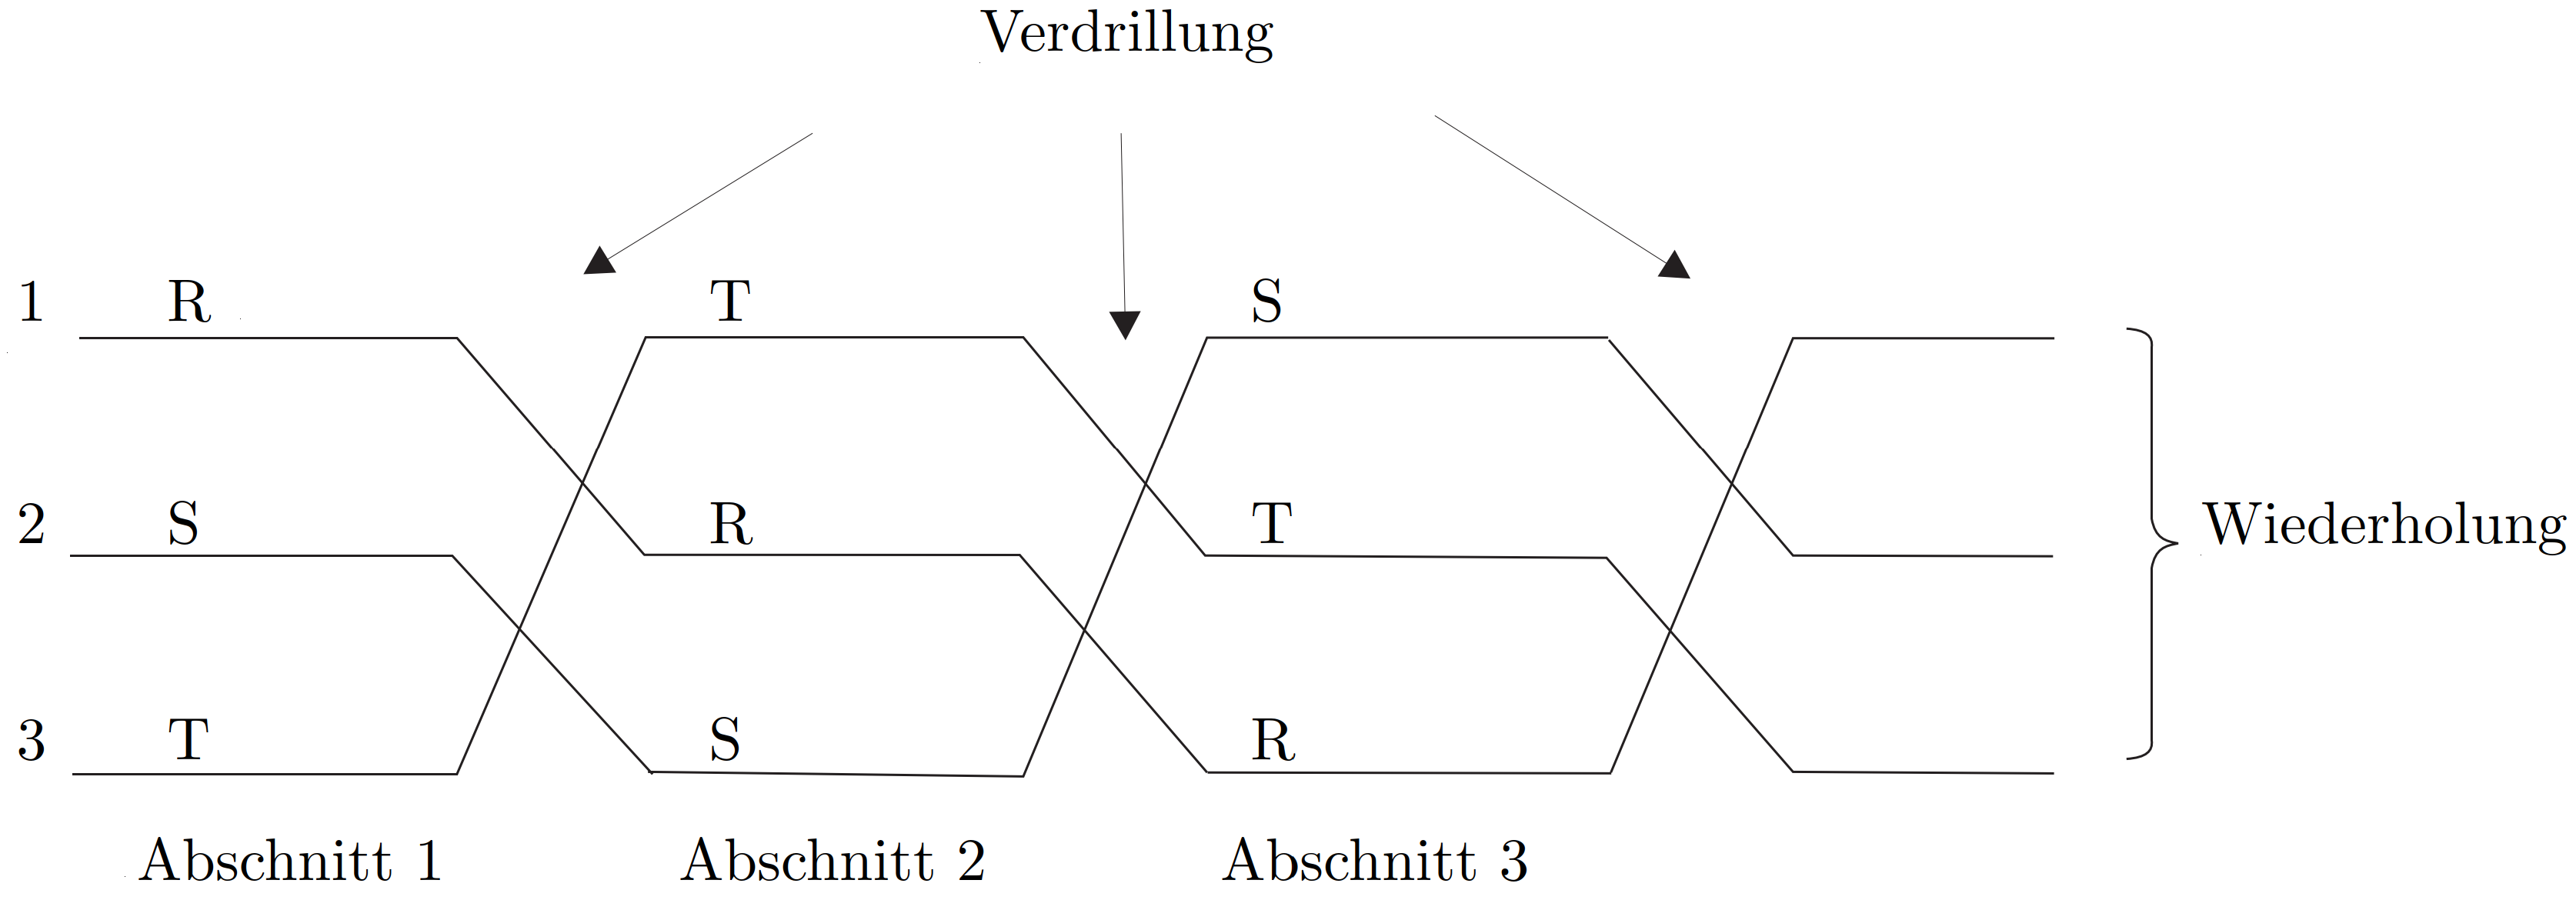
\includegraphics[width=0.98\columnwidth, align=c]{images/Verdrillung.png}

\vspace{0.15cm}

\begin{itemize}
    \item Die Leiterabstände sind bei einer Freileitung in der Regel nicht alle gleich.
    \item In Bezug auf die Koppelinduktivität ist die Leitung dann nicht symmetrisch.
    \item Man kann sie aber durch Phasentausch nach je einem Drittel der Leitungslänge symmetrisieren (verdrillen).
\end{itemize}


\subsection{Bündelleiter}

\includegraphics[width=0.98\columnwidth, align=c]{images/Bündelleiter.png}

\vspace{0.15cm}

$
\boxed{r_\text{eq} = \sqrt[n]{n \cdot R^{(n-1)} \cdot r}}
$

\vspace{0.15cm}

\renewcommand{\arraystretch}{1.2}
\begin{tabular}{@{} l p{8cm} l @{}}
$[r_\text{eq}]$ & Äquivalenter Leiterradius \dotfill & $\mathrm{m}$ \\
$[R]$           & Radius des Kreises, auf welchem die Bündelleiter angeordnet sind \dotfill & $\mathrm{m}$ \\
$[r]$           & Teilleiterradius \dotfill & $\mathrm{m}$ \\
$[n]$           & Anzahl der Bündelleiter \dotfill & $-$ \\
\end{tabular}
























